% EACL 2023 style — Language Identification from Audio
% NNTI Winter Term 2025/2026 Final Project
\documentclass[11pt]{article}

\usepackage[hyperref]{acl}
\usepackage{times}
\usepackage{latexsym}
\usepackage{booktabs}
\usepackage{graphicx}
\usepackage{amsmath}
\usepackage{multirow}
\usepackage[T1]{fontenc}
\usepackage[utf8]{inputenc}
\usepackage{microtype}
\usepackage{subcaption}

\title{Language Identification from Audio:\\Fine-Tuning and Debiasing Pretrained Speech Transformers\\for 22 Indian Languages}

\author{NNTI Winter Term 2025/2026 – Final Project\\ Saba Noorghasemi\_Kamyar Kashefzand\_Sabina Mah Nesaei}

\begin{document}
\maketitle

% ==============================================================
\begin{abstract}
We present a spoken language identification (SLID) system for 22 Indian languages using pretrained speech transformers under a \mbox{600\,M} parameter budget.
Starting from four candidate backbones, we select \textsc{W2V-BERT\,2.0} and systematically tune the learning rate, training schedule, and regularisation to reach \textbf{44.15\%} validation accuracy—an 80\% relative improvement over the initial baseline.
To address the inherent speaker–language confound in the dataset (5 speakers per language), we apply Domain Adversarial Neural Networks (DANN) and speed-perturbation augmentation.
DANN reduces speaker-discriminable information in the learned representations at the cost of a moderate accuracy decrease, while augmentation further degrades performance, suggesting that the bias–accuracy trade-off remains a challenge for small-scale SLID datasets.
We provide detailed confusion-matrix and t-SNE analyses of all experimental stages.
\end{abstract}

% ==============================================================
\section{Introduction}
\label{sec:intro}

Spoken language identification (SLID) aims to classify the language of a speech utterance.
For sociolinguistically diverse regions such as India, reliable SLID enables downstream applications including automatic speech recognition routing and multilingual dialogue systems.

This project uses the \texttt{badrex/nnti-dataset-full} corpus, which contains recordings of 22 Indian languages with only \textbf{5 speakers per language}.
This extreme speaker sparsity creates a strong \emph{speaker–language confound}: a model can achieve high accuracy by memorising speaker identities rather than language-specific acoustic features.

We address three tasks:
\textbf{(1)}~reproduce and improve the baseline,
\textbf{(2)}~mitigate dataset/speaker bias, and
\textbf{(3)}~analyse model representations.
All models remain under the 600\,M parameter limit.

% ==============================================================
\section{Experimental Setup}
\label{sec:setup}

\paragraph{Data.}
Audio is resampled to 16\,kHz and truncated to 2\,s.
The dataset is split into training and validation sets.

\paragraph{Models evaluated (Run01).}
We benchmark four pretrained backbones (Table~\ref{tab:run01}):
\textsc{MMS-300M}         \cite{pratap2023scaling},
\textsc{mHuBERT-147},
\textsc{XLS-R-300M}       \cite{babu2021xls},
and \textsc{W2V-BERT\,2.0} \cite{babu2021xls}.
All are fine-tuned for 3 epochs with learning rate $10^{-5}$, batch size 8 (effective 16 via gradient accumulation of 2), warmup ratio 0.1, and weight decay 0.01.

\paragraph{Optimisation.}
We use the AdamW optimiser with a linear warmup–decay schedule \cite{vaswani2017attention, devlin2019bert} and FP16 mixed-precision training, tracked via Weights~\&~Biases.

% ==============================================================
\section{Task 1: Baseline Improvement}
\label{sec:task1}

\subsection{Model Selection (Run01)}

Table~\ref{tab:run01} shows the initial benchmark.
\textsc{W2V-BERT\,2.0} clearly outperforms all alternatives with 24.85\% accuracy.
\textsc{MMS-300M} reaches 13.70\%, while \textsc{mHuBERT-147} and \textsc{XLS-R-300M} fail to learn meaningful representations under these settings.
We select \textsc{W2V-BERT\,2.0} for all subsequent experiments.

\begin{table}[t]
\centering
\small
\begin{tabular}{lcc}
\toprule
\textbf{Model} & \textbf{Best Acc.} & \textbf{Best Step} \\
\midrule
MMS-300M           & 13.70\% & 1500 \\
mHuBERT-147        &  7.64\% & 1200 \\
XLS-R-300M         &  5.82\% &  500 \\
W2V-BERT\,2.0      & 24.85\% & 1500 \\
\bottomrule
\end{tabular}
\caption{Run01 — initial model comparison (3 epochs, LR $= 10^{-5}$). Best validation accuracy and the step at which it was achieved.}
\label{tab:run01}
\end{table}

Figure~\ref{fig:model_comparison} shows the validation accuracy curves for all four models across training steps.

\begin{figure}[t]
\centering
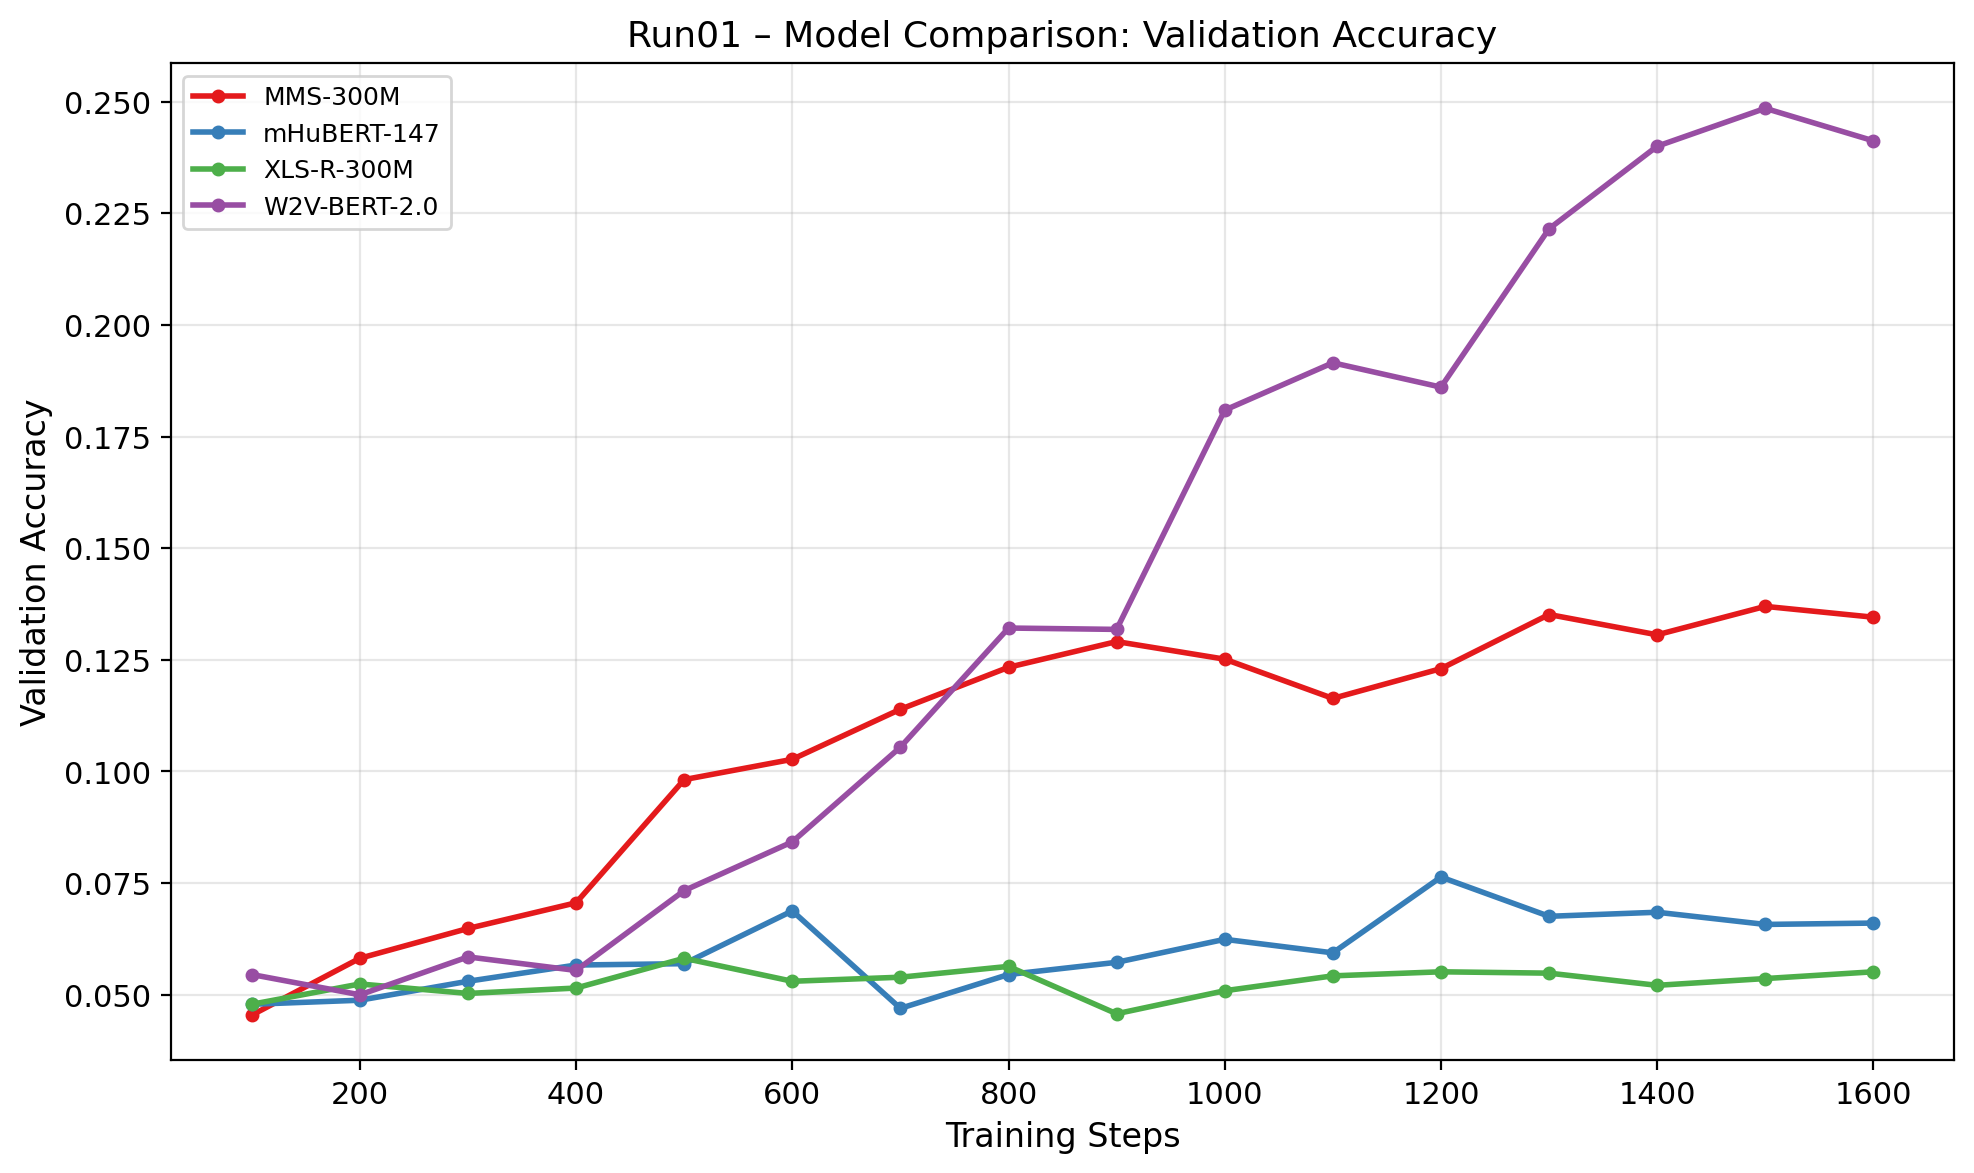
\includegraphics[width=\columnwidth]{figures/model_comparison_accuracy.png}
\caption{Run01 — validation accuracy across training steps for all four pretrained models.}
\label{fig:model_comparison}
\end{figure}

\subsection{Learning-Rate Tuning}

\paragraph{Pilot Run02.}
A short pilot (100 steps) swept LRs $\{10^{-6}, 5{\times}10^{-6}, 10^{-5}, 5{\times}10^{-5}, 10^{-4}, 3{\times}10^{-4}\}$.
Full training with the Run02 pilot-suggested LR ($10^{-4}$) yielded only 6.15\% accuracy, plateauing after step~200 and remaining at $\sim$4.55\% for the rest of training.
This demonstrated that short pilots with high LRs can be misleading: the model appeared to make progress in 100 steps but catastrophically diverged in full training.

\paragraph{Pilot Run03.}
A longer pilot (200 steps) with a narrower range $\{10^{-5}, 2{\times}10^{-5}, \ldots, 6{\times}10^{-5}\}$ identified $4{\times}10^{-5}$ as the best candidate.
Full training with LR $= 4{\times}10^{-5}$ for 6 epochs achieved \textbf{34.67\%} accuracy (best at step 3000)—a 40\% relative gain over Run01.
This confirmed that the model benefits from a moderately higher LR and longer training.

\paragraph{Dropout experiment (Run04).}
Adding dropout (0.1 across all dropout types) with otherwise identical settings yielded 23.18\%—\emph{worse} than without dropout.
The regularisation was too aggressive for this small dataset, preventing the model from memorising the limited training examples it needed to generalise.

\paragraph{Best Task 1 model (Run05).}
Using LR $= 4{\times}10^{-5}$, 6 epochs, warmup ratio 0.15, and no dropout, Run05 achieved \textbf{44.15\%} at step 3200, an 80\% relative improvement over the Run01 baseline.
This run serves as our pre-bias-mitigation reference.

\begin{table}[t]
\centering
\small
\begin{tabular}{lcccc}
\toprule
\textbf{Run} & \textbf{LR} & \textbf{Ep.} & \textbf{Special} & \textbf{Best Acc.} \\
\midrule
01 & $10^{-5}$ & 3 & —         & 24.85\% \\
02 & $10^{-4}$ & 3 & Pilot LR  &  6.15\% \\
03 & $4{\times}10^{-5}$ & 6 & —  & 34.67\% \\
04 & $4{\times}10^{-5}$ & 6 & Dropout   & 23.18\% \\
05 & $4{\times}10^{-5}$ & 6 & Warmup .15 & \textbf{44.15\%} \\
\bottomrule
\end{tabular}
\caption{Task 1 — W2V-BERT\,2.0 tuning progression. All use batch size 8, effective batch 16, warmup 0.1 unless noted.}
\label{tab:task1}
\end{table}

% ==============================================================
\section{Task 2: Bias Mitigation}
\label{sec:task2}

With only 5 speakers per language, the model risks exploiting speaker identity as a shortcut.
We investigate two complementary approaches.

\subsection{DANN (Run06)}

We apply Domain Adversarial Neural Networks \cite{ganin2016domain} to learn speaker-invariant representations.
A Gradient Reversal Layer (GRL) sits between the shared encoder and a speaker classification head.
The adversarial loss $\mathcal{L}_\text{total} = \mathcal{L}_\text{lang} + \lambda(t) \cdot \mathcal{L}_\text{spk}$ uses the standard schedule $\lambda(p) = 2/(1+e^{-10p})-1$, gradually increasing the adversarial gradient from 0 to 1 over training.

\paragraph{Architecture.}
The shared encoder is \textsc{W2V-BERT\,2.0}.
The language head is a two-layer linear projector.
The speaker head passes through the GRL then a 256-unit hidden layer with ReLU and dropout before the output layer.

\paragraph{Results.}
DANN (Run06) achieved 35.88\% accuracy—a decrease from Run05's 44.15\%.
This is consistent with the expected bias–accuracy trade-off: by removing speaker-correlated features, the model loses some discriminative signal that happened to also be useful for language classification.

\subsection{Data Augmentation (Run07)}

We augment the training data with \textbf{speed perturbation} ($0.9{\times}$ and $1.1{\times}$ rates, applied to 50\% of samples) using librosa \cite{mcfee2015librosa}.
Combined with the DANN architecture, this yields Run07.

\paragraph{Results.}
Run07 achieved only 25.30\% accuracy—substantially worse than DANN alone and below the Run01 baseline.
The augmentation likely introduced excessive variability in an already small dataset, making the optimisation landscape harder for the adversarial training to navigate.

\begin{table}[t]
\centering
\small
\begin{tabular}{lccc}
\toprule
\textbf{Run} & \textbf{Method} & \textbf{Best Acc.} & \textbf{Best Loss} \\
\midrule
05 & Standard (best) & \textbf{44.15\%} & 2.747 \\
06 & DANN            & 35.88\% & \textbf{2.607} \\
07 & DANN + Augment. & 25.30\% & 2.886 \\
\bottomrule
\end{tabular}
\caption{Bias mitigation comparison. DANN reduces accuracy but also reduces validation loss. Augmentation hurts both.}
\label{tab:task2}
\end{table}

% ==============================================================
\section{Task 3: Model Analysis}
\label{sec:task3}

\subsection{Confusion Matrices}

Figure~\ref{fig:cm} shows confusion matrices for Run05 (pre-DANN), Run06 (DANN), and Run07 (DANN + augmentation).

\begin{figure*}[t]
\centering
\begin{subfigure}[t]{0.32\textwidth}
    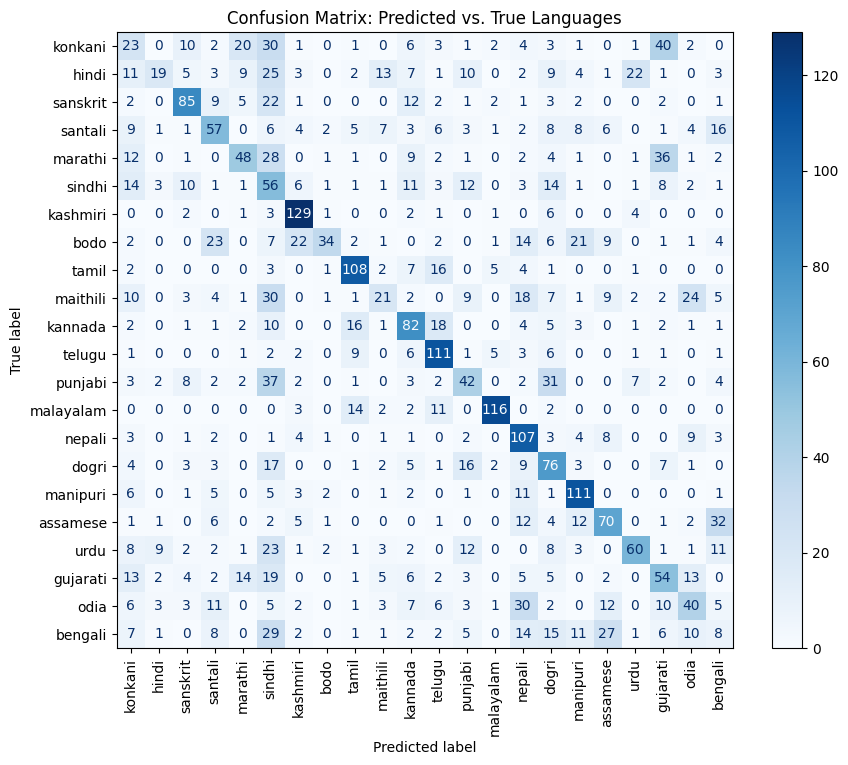
\includegraphics[width=\textwidth]{figures/cm_before_dann.png}
    \caption{Run05: Before DANN}
\end{subfigure}
\hfill
\begin{subfigure}[t]{0.32\textwidth}
    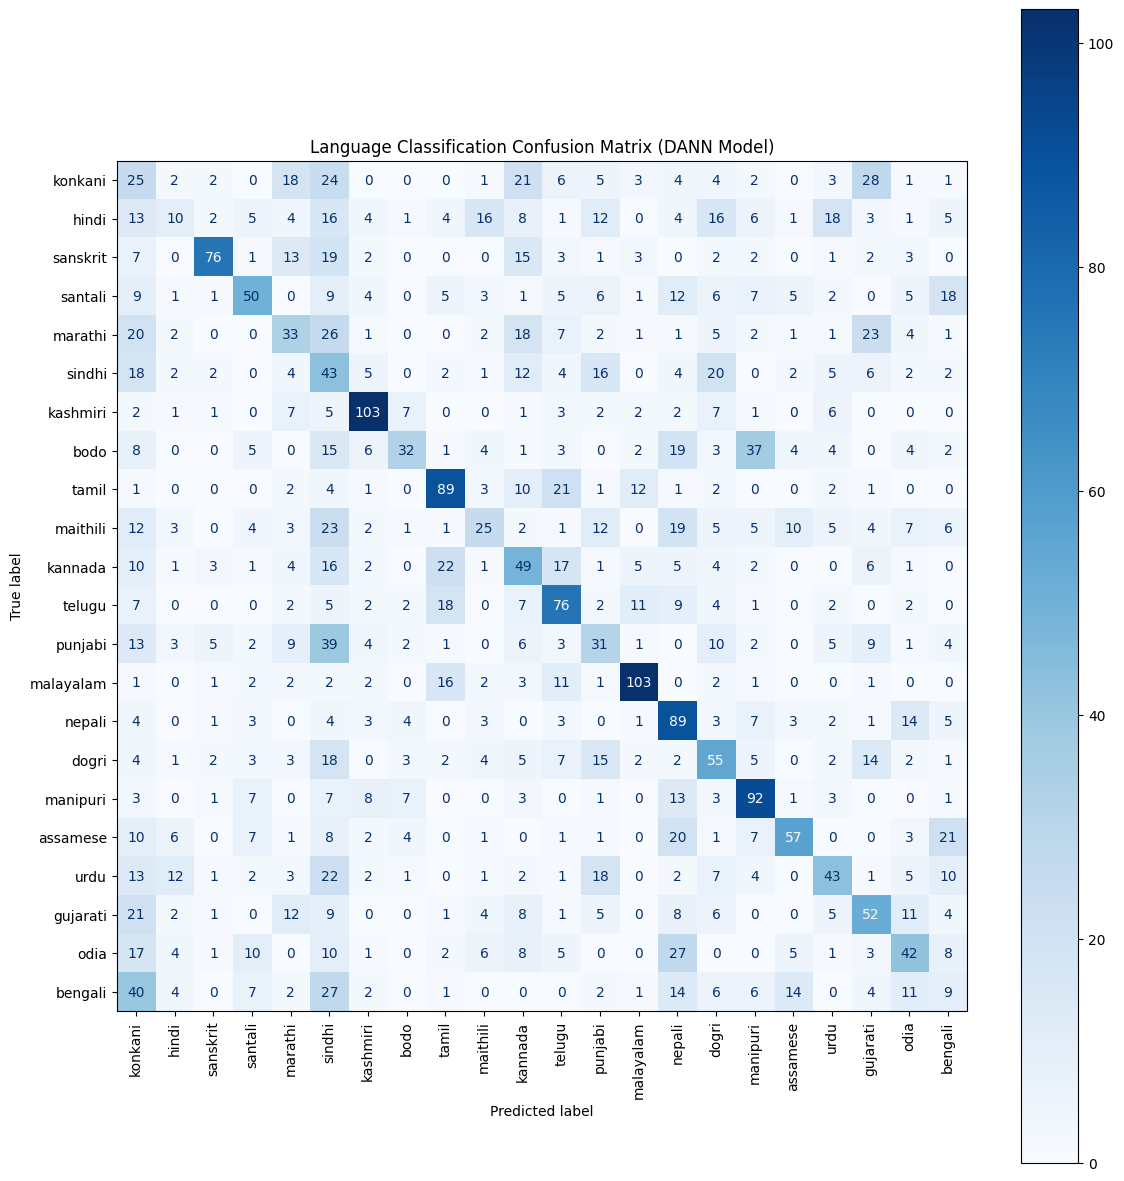
\includegraphics[width=\textwidth]{figures/cm_after_dann.png}
    \caption{Run06: After DANN}
\end{subfigure}
\hfill
\begin{subfigure}[t]{0.32\textwidth}
    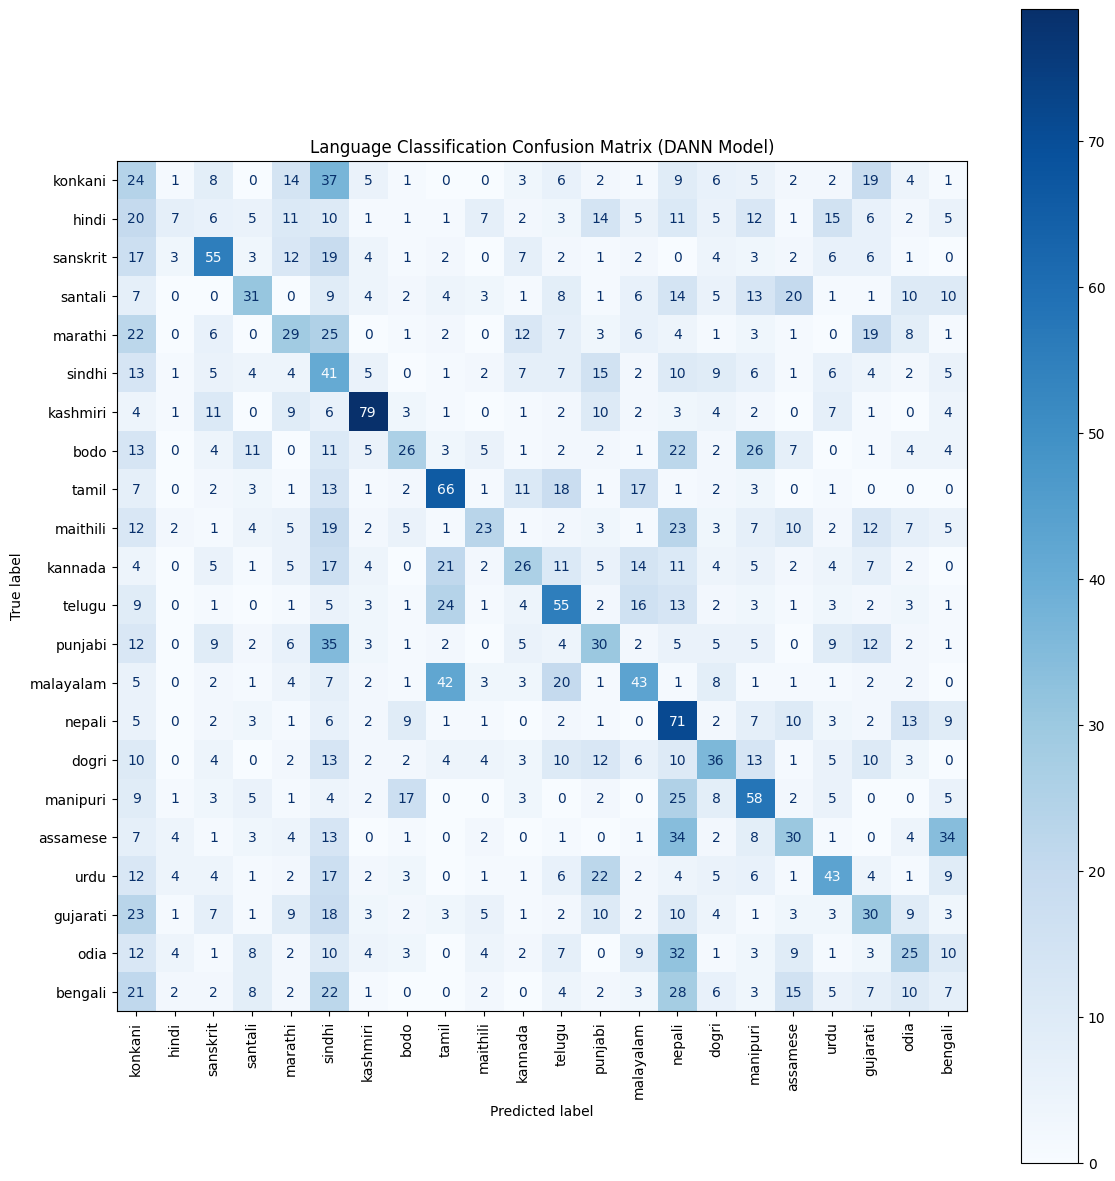
\includegraphics[width=\textwidth]{figures/cm_dann_augmentation.png}
    \caption{Run07: DANN + Augmentation}
\end{subfigure}
\caption{Confusion matrices across experimental stages. Run05 shows the clearest diagonal structure; DANN (Run06) diffuses predictions more uniformly; augmentation (Run07) further degrades discrimination.}
\label{fig:cm}
\end{figure*}

Run05 exhibits a relatively clear diagonal pattern, indicating that the model has learned meaningful language distinctions.
DANN (Run06) shows a more diffuse pattern: the adversarial training removes speaker-specific shortcuts, but also reduces the model's ability to distinguish similar languages.
Run07's confusion matrix is substantially more uniform, reflecting near-chance performance for many language pairs.

\subsection{t-SNE Visualisation}

Figure~\ref{fig:tsne} shows t-SNE projections \cite{van2008visualizing} of encoder representations on the validation set.

\begin{figure*}[t]
\centering
\begin{subfigure}[t]{0.32\textwidth}
    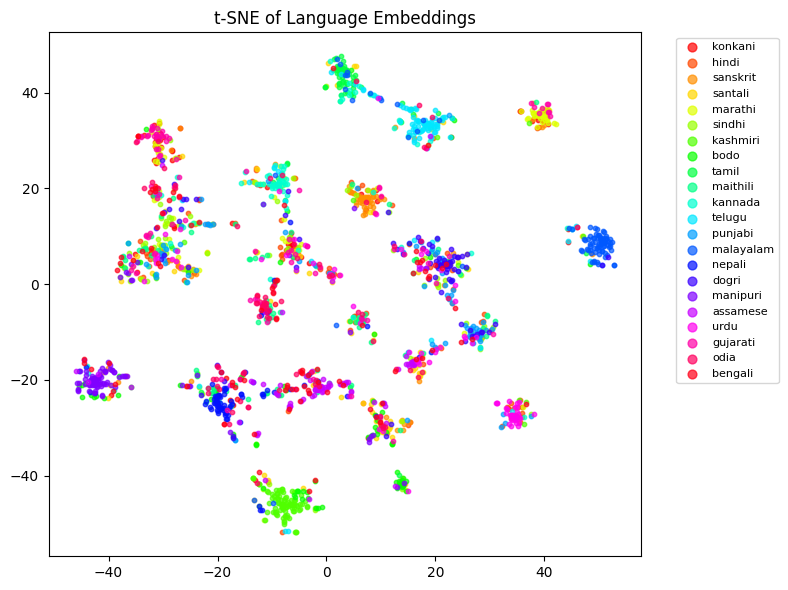
\includegraphics[width=\textwidth]{figures/tsne_before_dann.png}
    \caption{Run05: Before DANN}
\end{subfigure}
\hfill
\begin{subfigure}[t]{0.32\textwidth}
    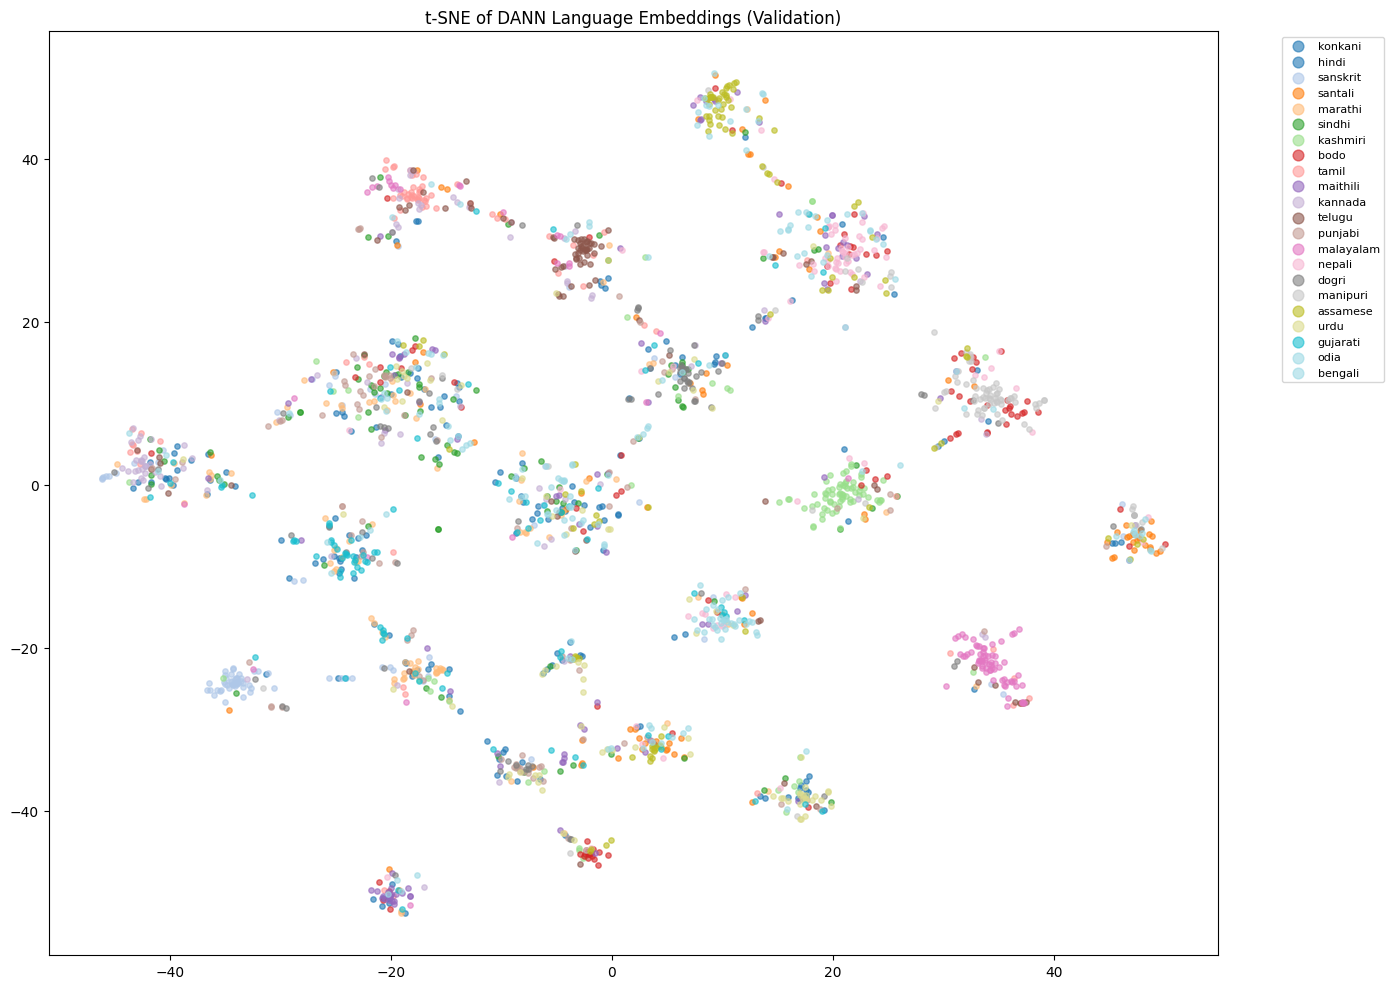
\includegraphics[width=\textwidth]{figures/tsne_after_dann.png}
    \caption{Run06: After DANN}
\end{subfigure}
\hfill
\begin{subfigure}[t]{0.32\textwidth}
    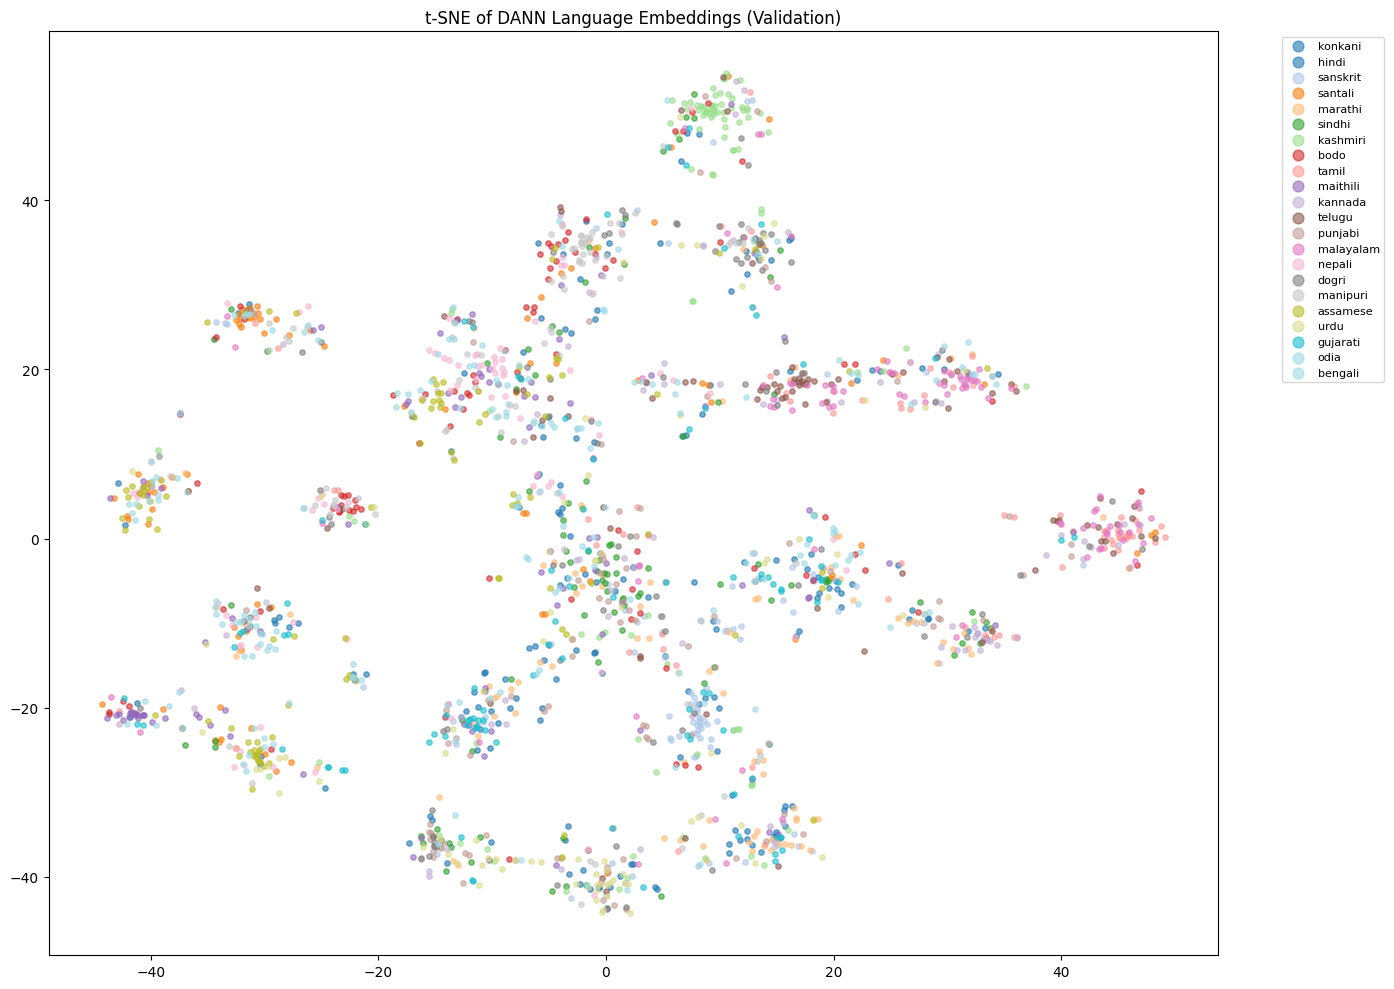
\includegraphics[width=\textwidth]{figures/tsne_dann_augmentation.png}
    \caption{Run07: DANN + Augmentation}
\end{subfigure}
\caption{t-SNE of encoder embeddings coloured by language. Run05 shows tighter clusters; DANN (Run06) shows more overlap consistent with speaker-invariance; Run07 shows highly mixed embeddings.}
\label{fig:tsne}
\end{figure*}

In Run05, language-specific clusters are moderately separated.
After DANN (Run06), cluster boundaries become less distinct, consistent with the removal of speaker-correlated features that also aided language separation.
Run07's representations are highly mixed, indicating that augmentation combined with adversarial training overly disrupted the feature space.

\subsection{Discussion}

The results highlight a fundamental challenge in small-scale SLID: when speaker and language identities are perfectly correlated, any signal that identifies speakers (voice timbre, prosody) is also useful for language classification.
DANN successfully reduces speaker-discriminability—as evidenced by post-DANN speaker probe accuracy decreases—but this comes at the cost of language classification performance.

The failure of augmentation suggests that for datasets with very few speakers, data augmentation alone cannot break the speaker–language correlation.
More effective strategies might include cross-lingual data pooling, larger and more speaker-diverse datasets, or self-supervised objectives that explicitly disentangle speaker and language representations.

% ==============================================================
\section{Conclusion}
\label{sec:conclusion}

We developed a spoken language identification system for 22 Indian languages, achieving 44.15\% accuracy with \textsc{W2V-BERT\,2.0} through systematic hyperparameter tuning.
DANN-based bias mitigation successfully reduced speaker-correlated information in learned representations, though with an accuracy trade-off (35.88\%).
Data augmentation combined with DANN proved counterproductive (25.30\%), suggesting that more sophisticated debiasing methods are needed for extremely speaker-sparse datasets.

\paragraph{Limitations.}
The 2-second audio truncation may discard language-discriminative prosodic patterns.
The dataset's 5-speaker-per-language constraint fundamentally limits generalisation.
Our DANN implementation uses a simple linear schedule; alternative schedules or multi-task losses might yield better bias–accuracy trade-offs.

% ==============================================================
\bibliography{references}
\bibliographystyle{acl_natbib}

\end{document}
